%!TEX root=masterproef.tex

\subsection{Semantisch model}
\label{subsection:devel-semantic-model}

De AST wordt door een eerste \emph{visitor} ingeladen in het SM. Dit is in
essentie een eenvoudige vertaling van de boomstructuur naar de overeenkomstige
elementen in het SM. Het resultaat kan opnieuw gevisualiseerd worden door
middel van GraphViz, zoals weergegeven in figuur \ref{fig:hello.sm}.

\begin{figure}[ht]
  \centering
  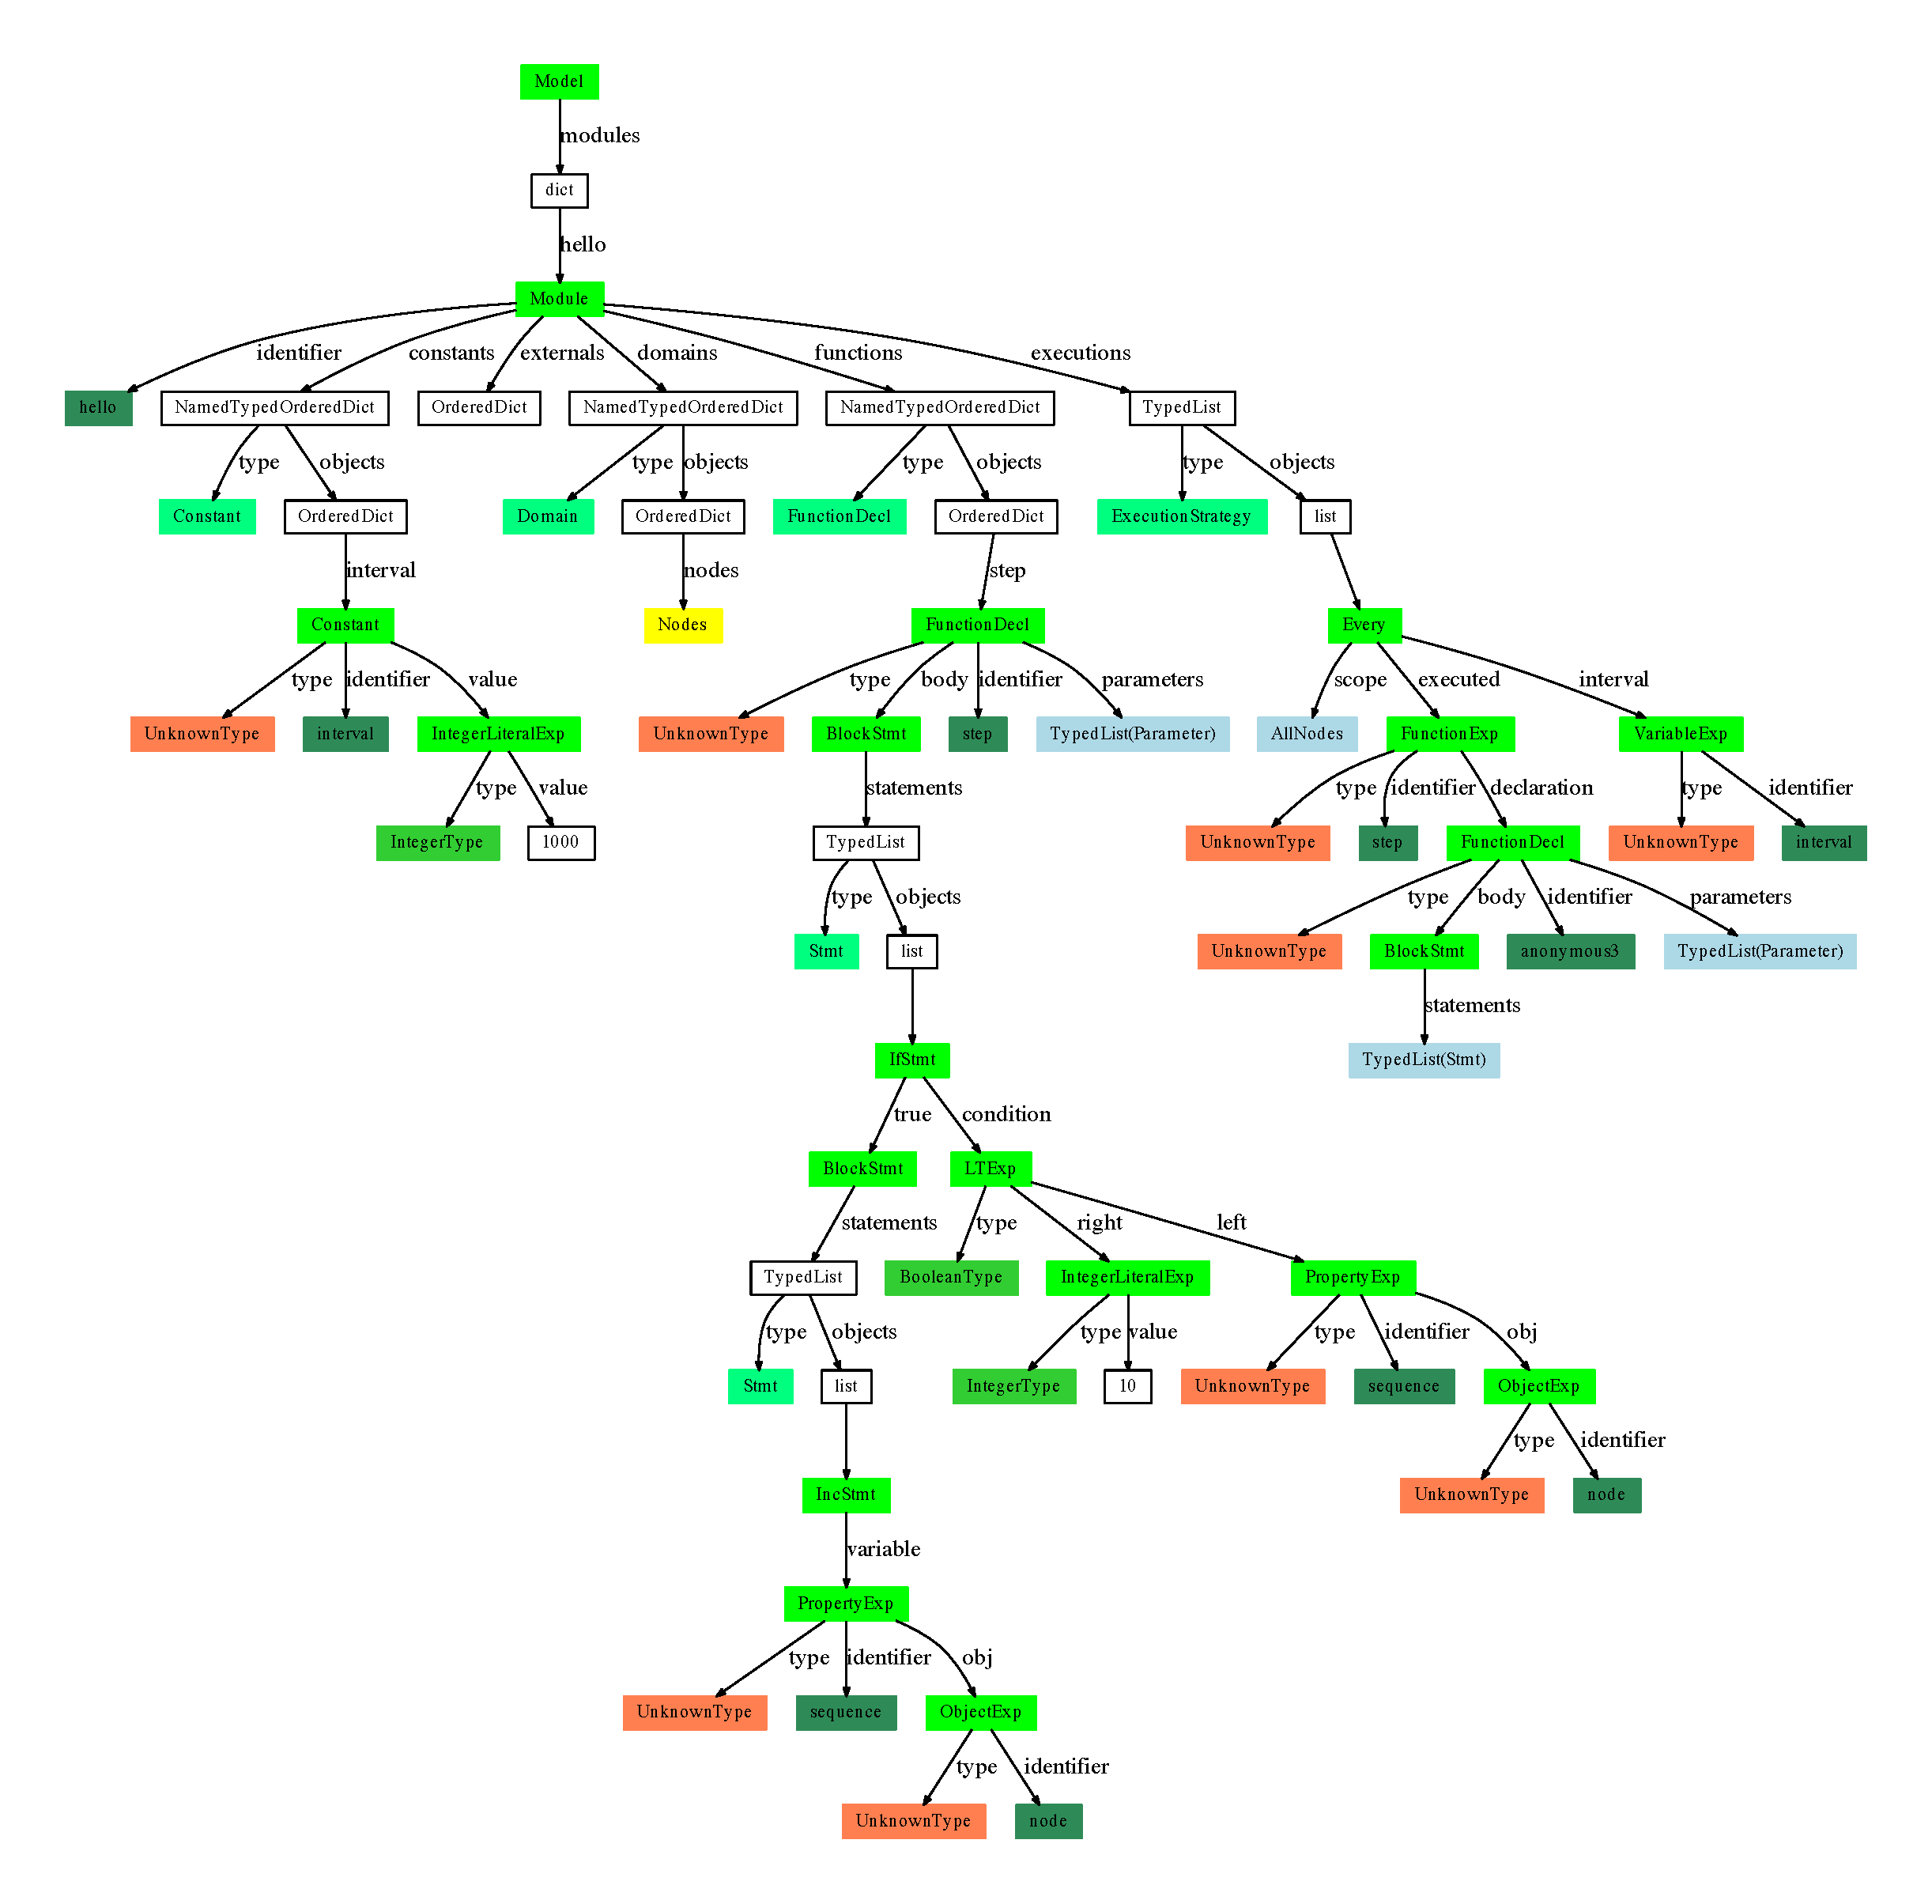
\includegraphics[width=\linewidth]{resources/hello_sm.pdf}
  \caption{Het SM van het elementaire voorbeeld, \ttt{hello.foo}}
  \label{fig:hello.sm}
\end{figure}

Bij deze visualisatie is gebruikgemaakt van een kleurencodering. Het SM kan
veel meer informatie bevatten dan de AST, zoals onder meer typering. Hierdoor
wordt de visualisatie van het SM ook een stuk groter. Dankzij de kleuren is het
makkelijker om het diagram te interpreteren.

De belangrijkste kleur is zonder meer de rode kleur. Deze geeft problemen aan
in het model. In dit geval betreft het onbekende types. Dit is in deze fase van
het generatieproces normaal aangezien typering in FOO-lang optioneel is. Deze
eerste versie van het SM bevat daarom nog niet alle types.

Een ander deel dat lijkt te ontbreken in dit diagram is de uitbreiding van het
domein. In het voorbeeld werd immers een eigenschap \ttt{sequence} toegevoegd.
Aangezien dit een uitbreiding is van het domein, zal deze terug te vinden zijn
in de eigen instantie van het domein voor deze module. In figuur
\ref{fig:hello.sm} is dit domein beperkt tot een referentie in een gele kleur.
De volledig inhoud van wat zich hierachter verschuilt, is opgenomen in bijlage
\ref{section:nodes.sm}.

Dit is een groot stuk van het SM en behelst verschillende types en functie
declaraties die door het knopendomein ge\"introduceerd worden in het SM. Hier
vinden we tevens de uitbreiding met de extra \ttt{sequence} eigenschap.

\subsubsection{Type deductie}

De volgende stap in het generatieproces bestaat erin om de nog onbekende types
te deduceren op basis van andere informatie uit het SM. Dit gebeurt aan de hand
van de \ttt{inferrer module}. Dit is een implementatie van de \emph{visitor}
voor het SM die nagaat dat alle types gekend zijn. Voor onbekende types wordt,
afhankelijk van de plaats van het type op verschillende manieren op zoek gegaan
naar een juiste typering.

De eenvoudigste methode bouwt terwijl het model doorlopen wordt een overzicht
op van gekende types die ontstaan door de declaratie van variabelen \dots
Indien een onbekend type wordt gevonden, consulteert de \ttt{inferrer module}
dit overzicht. Indien een referentie naar een eerdere declaratie gevonden
wordt, kan het type eenvoudig gededuceerd worden.

In een aantal gevallen is de deductie niet rechtstreeks af te lezen uit
eenvoudige declaraties en moet er naar andere mogelijke combinaties gekeken
worden. Voorbeelden hiervan zijn bv. functie declaraties die gebruikt worden
als reactie op een gebeurtenis. De gebeurtenis specificeert hoe de reagerende
functie gedeclareerd is. Op basis van de omkaderende gebeurtenis moet
vervolgens het overeenkomstige prototype van de functie opgezocht en gekoppeld
worden.

Na het succesvol uitvoeren van deze type deductie zijn de voordien onbekende
types gekend en is het model volledig. Figuur \ref{fig:hello.sm-inferred} toont
hetzelfde SM als voordien, echter nu met volledig gekende typering.

\begin{figure}[ht]
  \centering
  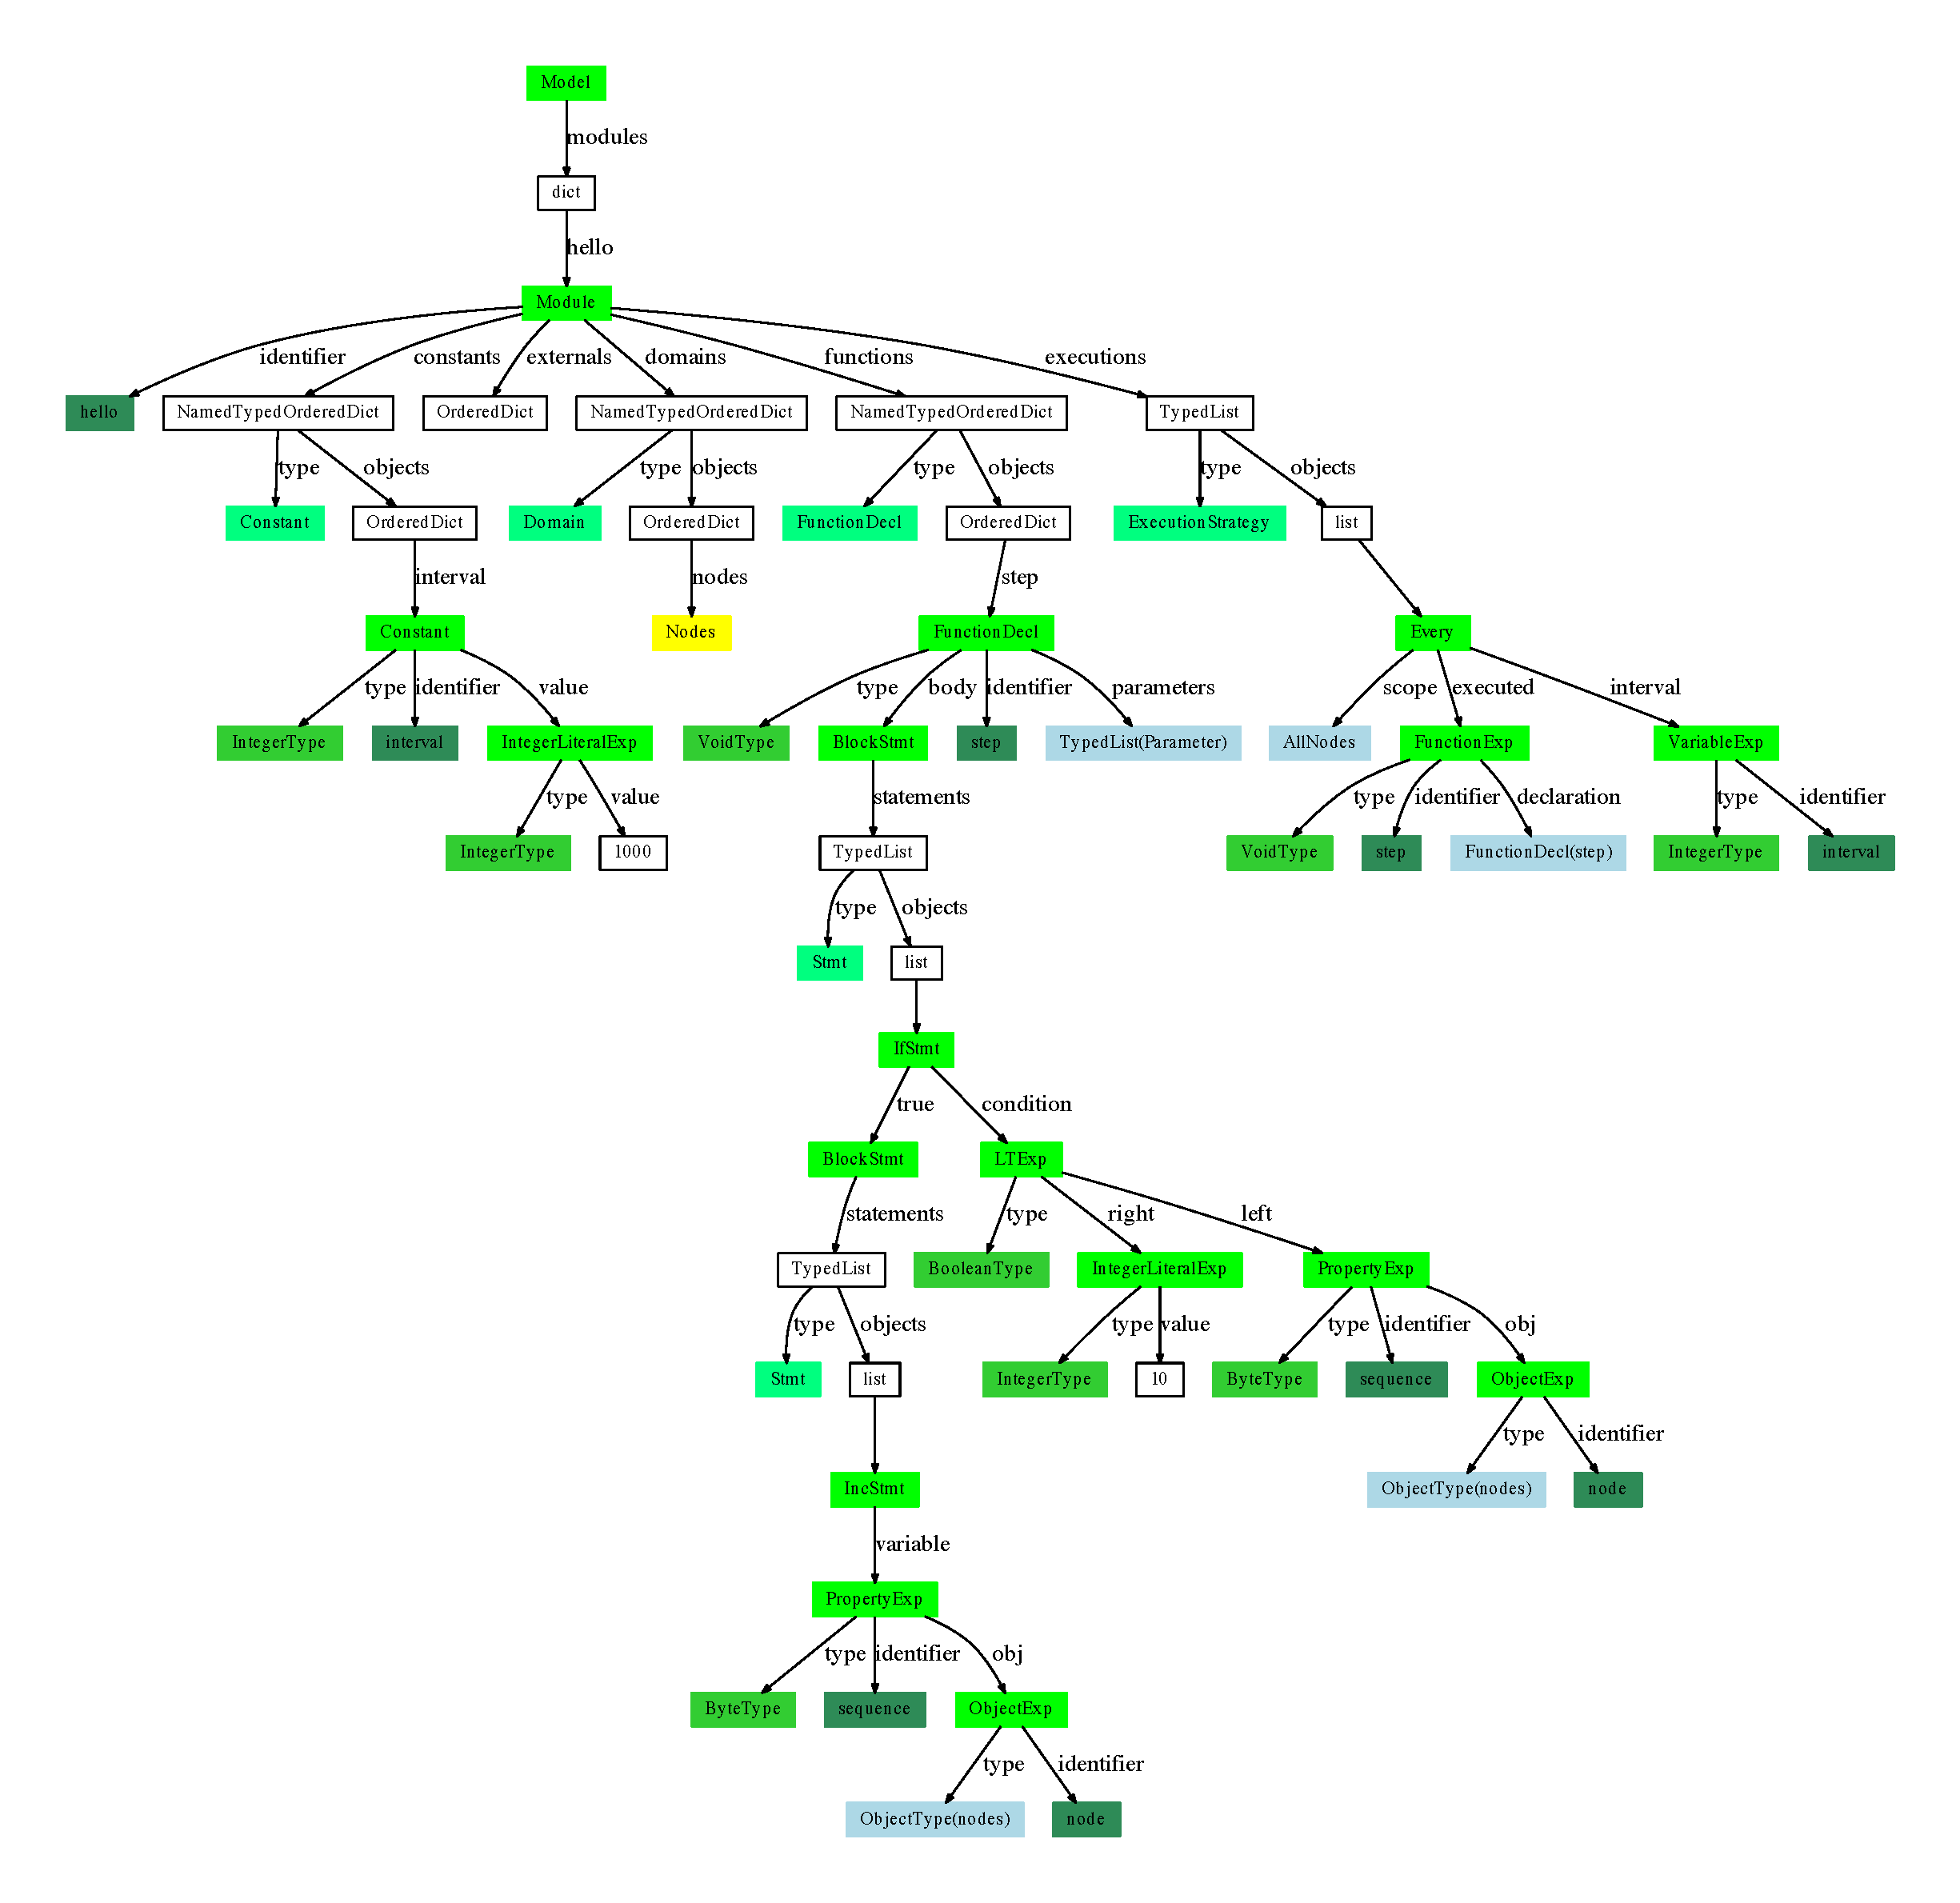
\includegraphics[width=\linewidth]{resources/hello_sm_inferred.pdf}
  \caption{Het SM van het elementaire voorbeeld, \ttt{hello.foo}, na type deductie}
  \label{fig:hello.sm-inferred}
\end{figure}

Ofschoon men verwacht dat deze fase geen structurele wijzigingen aanbrengt aan
het SM, zien we in dit geval toch dat er een vijftal elementen uit het model
verdwenen lijken te zijn. Dit is nochtans een gewoon voorbeeld van deductie. Na
het inladen van het initi\"ele model werd de (enige) uitvoeringsstrategie
gekoppeld aan een functie-expressie (\emph{FunctionExp}) genaamd, \ttt{step}.
Op dit ogenblik was er over step niets meer geweten. De declaratie van step was
wel eerder gebeurd, maar het is pas in de deductiefase dat het onbekende type
van deze functie opgezocht werd. Deel van het type is tevens de declaratie
ervan. Tijdens de deductie-fase wordt deze gekoppeld aan de eerdere declaratie,
waardoor dat in figuur \ref{fig:hello.sm-inferred} deze functiedeclaratie niet
meer volledig getoond wordt, maar nu als een referentie naar de \ttt{step}
functie opgenomen is.

\subsubsection{Model controle}

De \ttt{inferrer module} tracht alle onbekende types te deduceren. Hiermee
moeten normaal gezien de overblijvende problemen opgelost zijn. Een tweede
ondersteunende module is de \ttt{checker module} or model controle module. Deze
overloopt ook aan de hand van een \emph{visitor} het hele model en controleert
of alles in orde is.

De \ttt{checker module} is typisch nuttig bij het schrijven van FOO-lang code
en kan dienen als syntax en semantisch controle. Wanneer er bv. een schrijffout
gemaakt wordt in de naam van een variabele of functie, kan dit soms niet direct
opvallen. FOO-lang maakt bv. automatisch declaraties voor variabelen aan
wanneer zij voor het eerste gebruikt worden en nog niet eerder gedeclareerd
werden. De \ttt{checker module} kan bv. voor deze situaties waarschuwingen
geven, die kunnen helpen bij het schrijven van de FOO-lang broncode.
